\chapter{Аналитическая часть}

\section{Статический веб-сервер}

На самом базовом уровне, когда браузеру нужен файл, размещённый на веб-сервере, браузер запрашивает его через HTTP-протокол~\cite{mozilla_stserv}.
Когда запрос достигает нужного веб-сервера, HTTP-сервер принимает запрос, находит запрашиваемый документ и отправляет обратно также через HTTP~\cite{mozilla_stserv}.

Схема взаимодействия браузера и веб-сервера представлена на рисунке~\ref{serv_brow_rel}.
Статический веб-сервер посылает состоит из компьютера с HTTP-сервером и посылает размещенные в нем файлы в браузер без изменения их содержимого~\cite{mozilla_stserv}.

\begin{figure}[H]
	\centering
	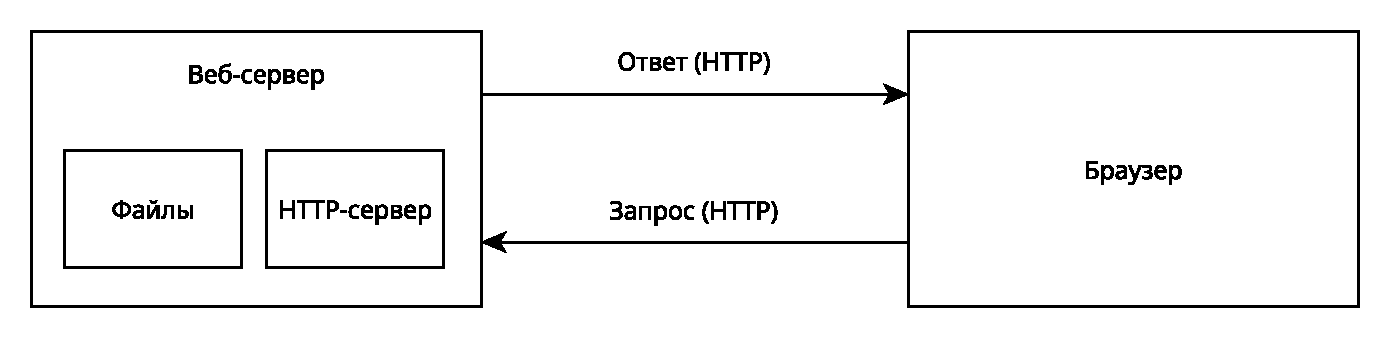
\includegraphics[width=\linewidth]{serv_brow_rel}
	\caption{Схема взаимодействия браузера и веб-сервера}
	\label{serv_brow_rel}
\end{figure}

\section{Протокол HTTP}

HTTP (Hypertext Transfer Protocol)~--- протокол прикладного уровня для передачи данных между узлами распределённых, объединённых, гипермедийных информационных систем~\cite{http}.
В основе HTTP лежит концепция <<клиент-сервер>>, то есть предполагается существование процессов-потребителей, которые инициируют соединение и посылают запрос, и процессов-поставщиков, которые ожидают соединения для получения запроса, производят необходимые действия и возвращают обратно сообщение с результатом~\cite{http}.

Протокол HTTP определяет два типа сообщений: запросы и ответы~\cite{http}.
Каждое HTTP-сообщение состоит из следующих элементов~\cite{http}:
\begin{itemize}
	\item стартовая строка,
	\item набор заголовков,
	\item тело.
\end{itemize}

Структура стартовой строки зависит от типа сообщения~\cite{http}.
В HTTP/1.1 стартовая строка запроса имеет следующий формат~\cite{http}:
\begin{center}
	<VERB>~<URI>~HTTP/1.1,
\end{center}
где VERB~--- тип запроса;\\
\text{~~~~~~}URI~--- идентификатор ресурса.

Стартовая строка ответа в HTTP/1.1 имеет следующую структуру~\cite{http}:
\begin{center}
	HTTP/1.1~<CODE>~<DESC>,
\end{center}
где CODE~--- код состояния ответа;\\
\text{~~~~~~}DESC~--- пояснение к коду ответа.

Код состояния ответа HTTP показывает, был ли успешно выполнен HTTP-запрос~\cite{http}.
В HTTP/1.1 приводится следующая классификация кодов состояния~\cite{http}:
\begin{itemize}
	\item информационные (100~--~199);
	\item успешные (200~--~299);
	\item перенаправления (300~--~399);
	\item клиентские ошибки (400~--~499);
	\item серверные ошибки (500~--~599).
\end{itemize}

Тип запроса (он же метод или глагол) определяет тип манипуляции над данными~\cite{http}.
В HTTP/1.1 существуют следующие глаголы~\cite{http}:
\begin{itemize}
	\item OPTIONS (описание параметров для соединения с ресурсом);
	\item GET (запрос представления данных);
	\item HEAD (запрос представления данных без тела ответа);
	\item POST (отправка сущностей к определенному ресурсу);
	\item PUT (замена всех текущих представлений ресурса данными запроса);
	\item DELETE (удаление указанного ресурса);
	\item TRACE (вызов возвращаемого тестового сообщения с ресурса);
	\item CONNECT (устанавливает <<туннель>> к серверу, определенному по ресурсу).
\end{itemize}

Заголовки HTTP позволяют клиенту и серверу отправлять дополнительную информацию с HTTP запросом или ответом~\cite{http}.
В HTTP-заголовке содержится нечувствительное к регистру название, а затем после символа двоеточия~--- непосредственно значение~\cite{http}.
Пробелы перед значением игнорируются~\cite{http}.

\section{Формализация бизнес-правил}

На рисунке~\ref{idef0} представлена формализация бизнес-правил разрабатываемого программного обеспечения в нотации IDEF0.
%\begin{figure}[H]
%	\centering
%	\includegraphics[width=\linewidth]{idef0}
%	\caption{Формализация бизес-правил разрабатываемого программного обеспечения}
%	\label{idef0}
%\end{figure}

\section*{Вывод}

Была изучена предметная область, связанная со статическим веб-сервером.
Был проведен анализ протокола HTTP.
Была осуществлена формализация бизнес-правил разрабатываемого программного обеспечения.

\clearpage